\chapter{Modellarchitektur und Ablauf}

In diesem Abschnitt wird der Aufbau und die Vorgehensweise des Algorithmuses bei SER-Systemen erläutert.


\section{2 Phasen der SER}

Die große Herausforderung für SER-Systemen ist die Unterscheidung der verschiedenen Emotionen durch die Sprache zu ermöglichen. Jeder Sprecher hat individuelle und kulturell bedingte Sprechstile, Sprechgeschwindigkeit, unterschiedliche Tonhöhe und Energiekontur im Spektrogramm, was das Extrahieren der Merkmale erschwert \cite{badshah2019deep}. Diese Umstände werden in der Verarbeitungseinheit behandelt, um später beim Klassifizieren der Sprachsignale gute Ergebnisse zu erhalten. 
\subsection{Verarbeitungseinheit (processing unit)}
Um die in 3.1 genannten Probleme anzugehen wird in der Verarbeitungseinheit das Spektrogramm in mehrere Blöcke (chunks) aufgeteilt, die Frames genannt werden (siehe Abbildung \ref{frames}) \cite{badshah2019deep}.
\begin{figure}[ht]
	\centering
	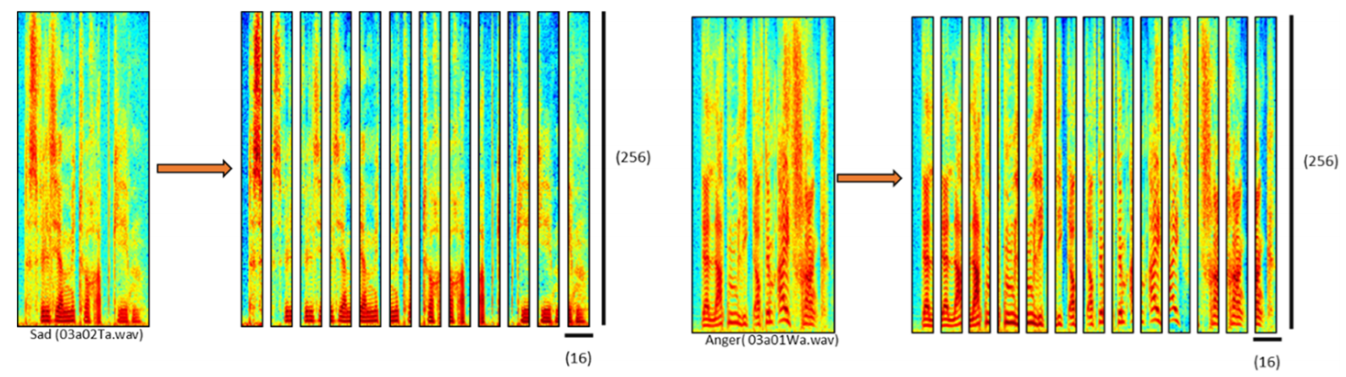
\includegraphics[width=1\textwidth]{images/frames}
	\caption{\label{frames} in Frames ausgeteilte Spektrogramme \cite{badshah2019deep}}
\end{figure}
\subsection{Klassifikator (classifier)}
Nachdem das Spektrogramm in mehreren Frames aufgeteilt wurde findet die Klassifikation mit Hilfe von Machine Learning Algorithmen statt \cite{badshah2019deep}. Hierbei werden die Frames einzeln untersucht und es kommen verschiedene Arten von Klassifikatoren zum Einsatz. Die gängigsten Algorithmen sind Hidden-Markov-Modelle (HMM), Gaußsches Mischungsmodell, Support Vector Machine (SVM), künstliche neuronale Netze und K-nearest neighbor, wobei SVM und HMM die am weitesten verbreiteten Lernalgorithmen für sprachbezogene Anwendungen sind \cite{badshah2019deep}.

\section{Aufbau der Modellarchitektur}


\begin{figure}[ht]
    \centering
    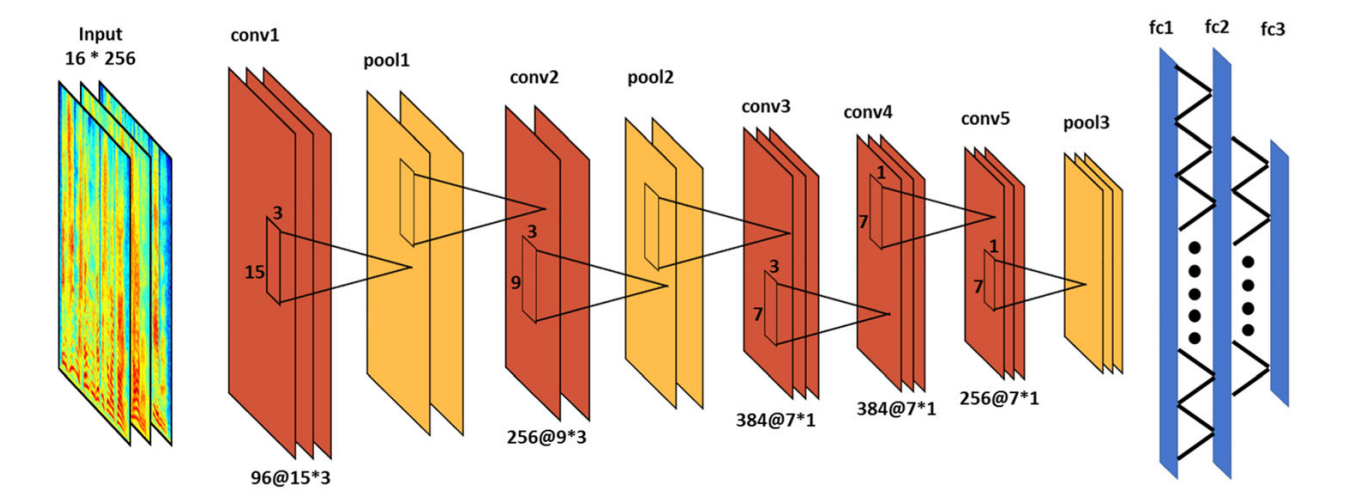
\includegraphics[width=1\textwidth]{images/conv}
    \caption{\label{architektur}CNN Architektur mit den unterschiedlichen Schichten \cite{badshah2019deep}}
\end{figure}

Mit Hilfe eines Labels kann man sich dann im Text auf diese Grafik (\ref{architektur}) beziehen. 



\section{Der Ablauf bei SER}

\begin{figure}[ht]
	\centering
	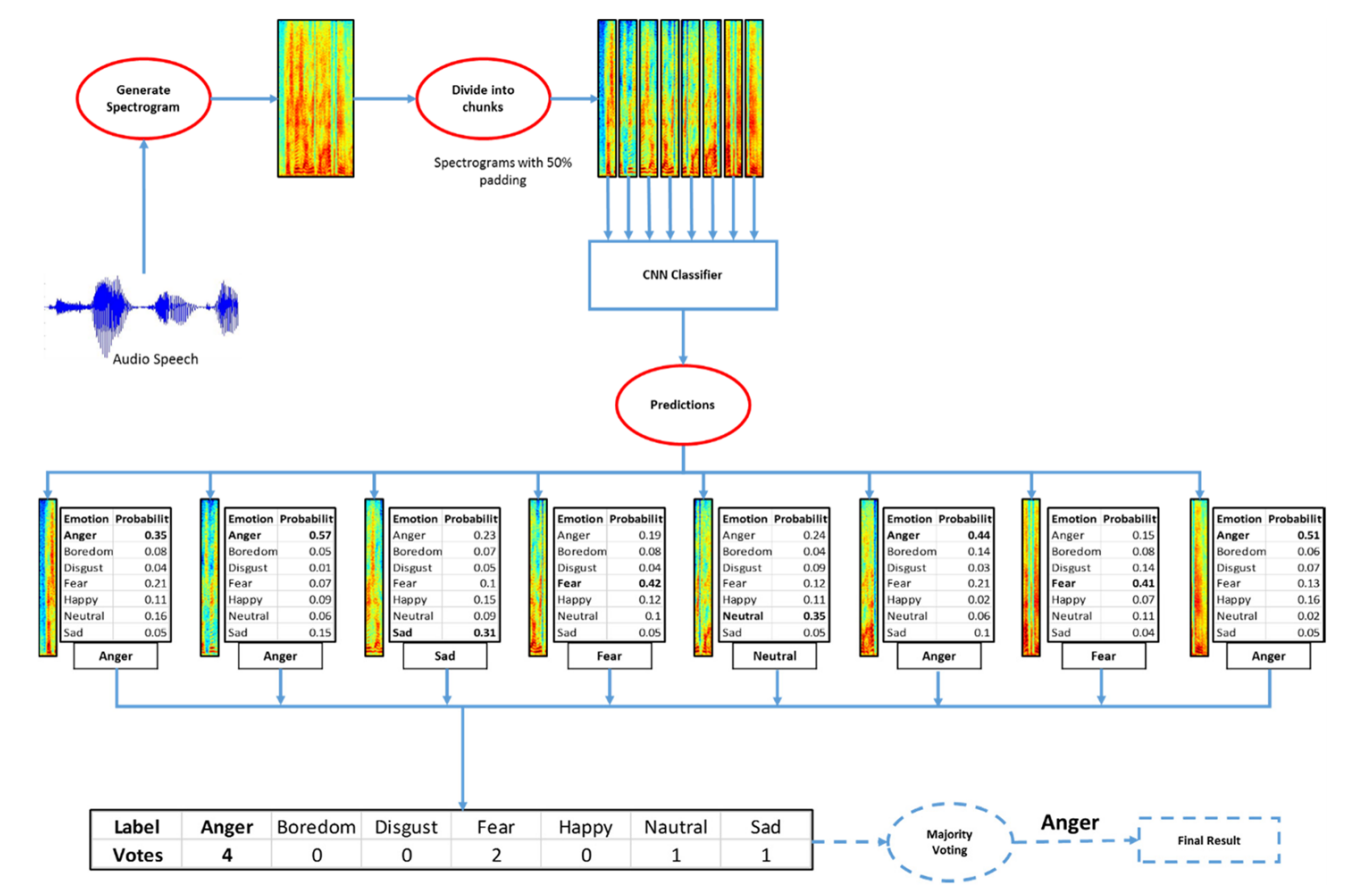
\includegraphics[width=1\textwidth]{images/ablauf}
	\caption{\label{ablauf}spezifischer Schema und Ablauf bei SER \cite{badshah2019deep}}
\end{figure}




